\subsubsection{Die Bibliothek \emph{gdata}}
Die Google-Bibliothek \emph{gdata} ist eine frei verf\"ugbare Bibliothek zum erstellen von
 Clientapplications für die Services der Google-Cloud.
\emph{gdata} kapselt die Webservices komplett in Java-Klassen, so dass ein importieren
 (z.\ B.\ mit \emph{wsimport}) nicht mehr notwendig ist.

\subsubsection{Authentifizieren und Verbinden mit \emph{gdata}}
Google bietet zwei Authentifizierungsverfahren an
\begin{enumerate}
	\item\emph{OAuth}
	\item Username und Passwort
\end{enumerate}
\emph{OAuth} ist ein Service, der bei erfolgreicher Anmeldung ein Token erstellt, mit dem
 der Client von Google bereitgestellte Services aufrufen und sich authentifizieren kann.
So muss der Client die Anmelde-Daten des Nutzers nicht speichern, sondern nur den Token.
In Abbildung \ref{fig:google_oauth} wird ein Beispiel für die Nutzung von \emph{OAuth} dargestellt.
% TODO Quelle https://developers.google.com/accounts/docs/OAuth2
\begin{figure}[h!]
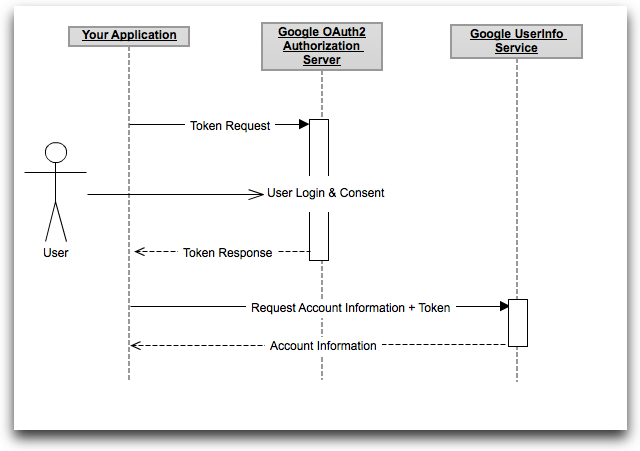
\includegraphics[width=\textwidth]{Bilder/google_oauth.png}
\label{fig:google_oauth}
\caption
\end{figure}

Da wir unseren eigenen Account nutzen und die Daten nicht Sicherheitskritisch sind, haben
 wir die zweite Variante gewählt und authentifizieren uns bei jedem Service-Aufruf mit
 Username und Passwort.

\subsubsection{Kontakte suchen}

\subsubsection{Kontakte einf\"ugen}